% flashcards-title: Dot plot of six repeated length readings
% flashcards-desc: A number line of lengths in centimeters runs from twelve to thirteen, with labeled marks at every two tenths and small unlabeled steps at every tenth. Six filled dots sit above the line, one per recorded reading, with equal readings stacked vertically. Five dots gather between the twelve point three and twelve point five positions, stacking three high at one value, while a single dot sits alone farther to the right near the twelve point nine position.
\documentclass[dvisvgm,tikz,border=8pt]{standalone}
\usepackage{tikz}
\usetikzlibrary{arrows.meta,calc,positioning}
\definecolor{DeckInk}{HTML}{172A3A}
\definecolor{DeckAccent}{HTML}{176B87}
\definecolor{DeckWarm}{HTML}{D97706}
\definecolor{DeckMuted}{HTML}{667784}
\definecolor{DeckPaper}{HTML}{F7FAFC}
\tikzset{
  every node/.style={font=\sffamily, text=DeckInk},
  object/.style={draw=DeckInk, line width=1.1pt, fill=DeckPaper},
  primary/.style={draw=DeckAccent, line width=1.5pt},
  boundary/.style={draw=DeckAccent, line width=1.5pt, dashed, rounded corners=6pt},
  guide/.style={draw=DeckMuted, line width=0.9pt, dashed},
  dimension/.style={{Stealth[length=3.2mm,width=2.2mm]}-{Stealth[length=3.2mm,width=2.2mm]}, draw=DeckWarm, line width=1.2pt},
  motion/.style={-{Stealth[length=3.5mm,width=2.5mm]}, draw=DeckAccent, line width=1.5pt, dashed},
}

\begin{document}
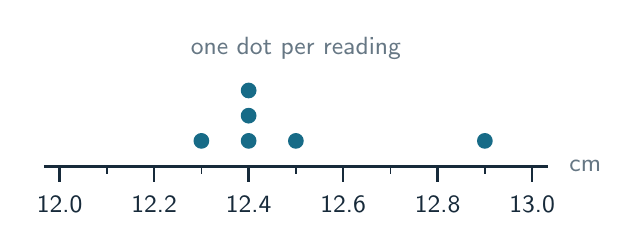
\begin{tikzpicture}[x=1cm,y=1cm]
  % Axis: x = (value - 12.0) * 6
  \draw[DeckInk, line width=1.1pt] (-0.2,0) -- (6.2,0);
  \foreach \x in {0,0.6,...,6.0}
    \draw[DeckInk, line width=0.5pt] (\x,0) -- (\x,-0.1);
  \foreach \x/\v in {0/12.0, 1.2/12.2, 2.4/12.4, 3.6/12.6, 4.8/12.8, 6.0/13.0}{
    \draw[DeckInk, line width=0.9pt] (\x,0) -- (\x,-0.2);
    \node[font=\sffamily\small] at (\x,-0.48) {\v};
  }
  \node[font=\sffamily\small, text=DeckMuted, anchor=west] at (6.35,0) {cm};
  % Readings: 12.3, 12.4 (x3), 12.5, 12.9
  \fill[DeckAccent] (1.8,0.32) circle (0.1);
  \fill[DeckAccent] (2.4,0.32) circle (0.1);
  \fill[DeckAccent] (2.4,0.64) circle (0.1);
  \fill[DeckAccent] (2.4,0.96) circle (0.1);
  \fill[DeckAccent] (3.0,0.32) circle (0.1);
  \fill[DeckAccent] (5.4,0.32) circle (0.1);
  \node[font=\sffamily\small, text=DeckMuted] at (3.0,1.5) {one dot per reading};
\end{tikzpicture}
\end{document}
